% \documentclass{WHUBachelor}% 选项 forprint: 交付打印时添加, 避免彩色链接字迹打印偏淡. 即使用下一行:
\documentclass[forprint]{myreport}
\usepackage{tcolorbox}

%\usepackage{listings}
\lstdefinestyle{lfonts}{
  basicstyle = \footnotesize\ttfamily,
  stringstyle = \color{purple},
  keywordstyle = \color{blue!60!black}\bfseries,
  commentstyle = \color{olive}\scshape,
}
\lstdefinestyle{lnumbers}{
  numbers = left,
  numberstyle = \tiny,
  numbersep = 1em,
  firstnumber = 1,
  stepnumber = 1,
}
\lstdefinestyle{llayout}{
  breaklines = true,
  tabsize = 2,
  columns = flexible,
}
\lstdefinestyle{lgeometry}{
  xleftmargin = 20pt,
  xrightmargin = 0pt,
  frame = tb,
  framesep = \fboxsep,
  framexleftmargin = 20pt,
}
\lstdefinestyle{lgeneral}{
  style = lfonts,
  style = lnumbers,
  style = llayout,
  style = lgeometry,
}
\lstdefinestyle{c}{
	language = {c},
	style = lgeneral,
}



\begin{document}
%%%%%%%%%%%%%%%%%%%%%%%%%%%%%%%%%%%%%%%%%%%%%%%%%%%%%%%%%%%%%%%%%%%%%%%%%%%%
% 封面
%%%%%%%%%%%%%%%%%%%%%%%%%%%%%%%%%%%%%%%%%%%%%%%%%%%%%%%%%%%%%%%%%%%%%%%%%%%%
\title{ 基于物品的协同过滤推荐算法 \\ 集群部署及算法实现}
\Cschoolname{数据科学与计算机学院}          % 学院名
\Cmajor{计算机科学与技术}                  % 专业中文名
\StudentNumber{16337237} % 填写自己的学号
\author{王永锋}                            % 作者名字
\Csupervisor{陈鹏飞}        %指导教师中文名、职称
\date{二〇一八年七月一日}                % 日期, 要注意和英文日期一致!!
\pdfbookmark[0]{封面}{title}         % 封面页加到 pdf 书签
\maketitle
\frontmatter
%%%%%%%%%%%%%%%%%%%%%%%%%%%%%%%%%%%%%%%%%%%%%%%%%%%%%%%%%%%%%%%%%%%%%%%%%%%%
% 目录
%%%%%%%%%%%%%%%%%%%%%%%%%%%%%%%%%%%%%%%%%%%%%%%%%%%%%%%%%%%%%%%%%%%%%%%%%%%%
% 把目录加入到书签
\pagenumbering{Roman}              % 正文之前的页码用大写罗马字母编号.
\pdfbookmark[0]{目录}{toc}
\tableofcontents
%% 以下是正文
\mainmatter 
%%%%%%%%%%%%%%%%%%%%%%%%%%%%%%%%%%%%%%%%%%%%%%%%%%%%%%%%%%%%%%%%%%%%%%%%%%%%
% 正文
%%%%%%%%%%%%%%%%%%%%%%%%%%%%%%%%%%%%%%%%%%%%%%%%%%%%%%%%%%%%%%%%%%%%%%%%%%%%

\chapter{项目概述}

在《并行与分布式》的课程项目中,我使用自己与同学的3台多余的电脑,在宿舍搭建了一个hadoop集群,并在该集群上运行我们编写的hadoop任务。同时,我参考教程,编写了适用于hadoo1.2.1的基于物品的协同过滤推荐算法java实现。

为了测试我们搭建的集群能否做到并行与分布式的使用Mapreduce的方法计算数据,我们从\url{https://grouplens.org/datasets/movielens/}上下载到了与推荐电影相关的数据,并从中提取了前30万行放到hdfs分布式文件系统中进行计算,经过了10小时的计算后,我成功的得到了推荐的结果。

在完成项目的过程中,我在配置还有计算的时候也遇到了一些问题,具体的细节会在下面详细说明。

\chapter{集群部署}

\subsection{网络环境}

我和同学的三台笔记本,通过极路由1s相连,具体细节可见表\autoref{tab:}

%\usepackage[svgnames,table]{xcolor}
%\usepackage{changepage}
%\usepackage{rotating}
%\begin{sidewaystable}[htp]
\begin{table}[htp]
  \caption{主机IP地址}
  \centering
  \rowcolors{1}{White}{Lavender}
  %\begin{adjustwidth}{-1.5cm}{-1cm}
  \begin{tabular}{cccp{11cm}<{\centering}}
%\multicolumn{2}{c}{contents}
%\usepackage{booktabs}
%\cmidrule{2-3}
  \toprule
    主机名 & IP 地址 & 与路由器相连方式 \\
  \midrule
    wyf-ubuntu-server & 192.168.199.177 & 通过wifi相连 \\
    yb-ubuntu-server & 192.168.199.133 & 通过网线相连 \\
    lxr-ubuntu-server & 192.168.199.248 & 通过网线相连\\
  \bottomrule
  \hiderowcolors
  \end{tabular}
  %\end{adjustwidth}
  \label{tab:deploy-1}
\end{table}


%\usepackage{tcolorbox}
%\newtcolorbox{mybox}{}
%\renewtcolorbox{mybox}{colback = red!25!white, colframe = red!75!black}
%\begin{mybox}[title = {}]
\begin{tcolorbox}[title = {有关网络环境的一些思考}]
关于无线网络与有线网络的对比。
\tcblower

一开始我们是有两台电脑都通过无线wifi来进行连接,但由于无线链路由于众所周知的原因,带宽并不如有线链路。因此出现局域网内速度总是这相当多的瓶颈。

出现这问题的主要原因是,作为一个分布式集群,集群内的电脑中的分布式文件系统需要通过不断的向局域网中的其他主机发送或接受文件,这对局域网的要求是很高的。一般的家用路由器对局域网内的网络支持并不如专业的交换机良好,网络链路更是容易受到信道容量的限制,集群之间的电脑通信延迟增大,大大降低了分布式集群的性能。


\end{tcolorbox}

TODO:如果有当时的网速截图就好了


\subsection{主机的配置}


每一台主机配置hadoop环境的过程,其实网络上都已经说了很多了,也有很多教程帮助我们最终成功配置好了集群,跑起了数单词的程序,并最终得出了正确答案。下面简单说一下配置过程,还有说一下配置过程中遇到的一些问题。

在主节点上的配置

\begin{itemize}
  \item 安装jdk,并设置环境变量
  \item 下载hadoop1.2.1编译后的包
  \item 编辑$\backslash$etc$\backslash$hosts文件,方便使用主机名作为每一台主机的标识而不是ip地址
  \item 分别配置hadoop1.2.1下conf文件夹中的core-site.xml,mapred-site.xml,hdfs-site.xml
  \item 配置hadoop-env.sh 文件中的JAVA\_HOME变量
  \item 编辑masters和slaves文件
  \item 格式化文件系统
  \item 将配置文件分发到每台slaves上
  \item 执行start-all.sh脚本,启动服务器
\end{itemize}

%\usepackage{tcolorbox}
%\newtcolorbox{mybox}{}
%\renewtcolorbox{mybox}{colback = red!25!white, colframe = red!75!black}
%\begin{mybox}[title = {}]
\begin{tcolorbox}[title = {配置过程中出现的一些问题}]
我们在配置的过程中, 有两个问题花了很长时间才解决好。
\tcblower

\begin{itemize}
  \item 无论如何配置,都无法启动datanotes
  \begin{itemize}
    \item 删除了master和slaves上的hadoop目录下的所有数据,就可以解决。
    \item 猜测是因为如果不删除旧的文件,一些过去的配置无法被刷新。
  \end{itemize}
  \item 主节点不能够参与运算
  \begin{itemize}
    \item 是我自己没有想清楚,其实只需要在slaves中写上master节点的主机名,就能够做到master节点同样参与运算。
  \end{itemize}
\end{itemize}

\end{tcolorbox}

\chapter{算法原理与实现}

我们实现的算法是基于物品的协同过滤推荐算法,这个算法的核心是矩阵相乘。因此,在明确了算法原理后,我们使用了mapreduce将输入的用户评分数据进行预处理,矩阵相乘。为了实现最终得到推荐的分数,我们使用了5步mapreduce来实现。

这一个系统的输入与输出如下:

输入:每一行形如 UserID,FilmID,Score
其中UserID为用户ID,FilmID为电影ID,Score为评分。

输出:每一行形如UserID d1\_s1,d2\_s2,d3\_s3。
其中UserID为用户ID,与输入数据对应,随着UserID之后的列表,d(n)为电影ID,s(n)为预测的该用户对该电影的评分。注意到后面的电影ID应该都是该用户没有看过的电影。

\section{实现原理}

我们使用了五步Mapreduce来实现这一个推荐系统。

\subsection{每一步的大致作用}

TODO:这里需要说每一步的mapreduce的大致作用,让读者对整个过程有个大致的了解。

\section{实现细节}



\subsection{第一步}

TODO:数据预处理

\subsection{第二步}

TODO:计算相似度矩阵

\subsection{第三步}

TODO:矩阵转置

\subsection{第四步}

TODO:矩阵相乘

\subsection{第五步}

TODO: 去除已看过电影数据


\chapter{测试结果}

在完成代码后,我们先拿了简单的数据测试,保证代码功能的正确性,然后我们使用的来自一网站\url{https://grouplens.org/datasets/movielens/}的公开数据集,提取了前30万行数据进行计算。

计算的过程可见\autoref{fig:result-step4-top},同时,与此对应的,在hadoop管理页面上可见jobtracker的情况,如\autoref{fig:result-step4-jobtracker}。

%\usepackage{changepage}
%\usepackage{rotating}
%\usepackage{float}
%\usepackage[section]{placeins}
%\begin{sidewaystable}[!Htp]
\begin{figure}[htp]
  %\begin{adjustwidth}{-1.5cm}{-1cm}
  \centering
  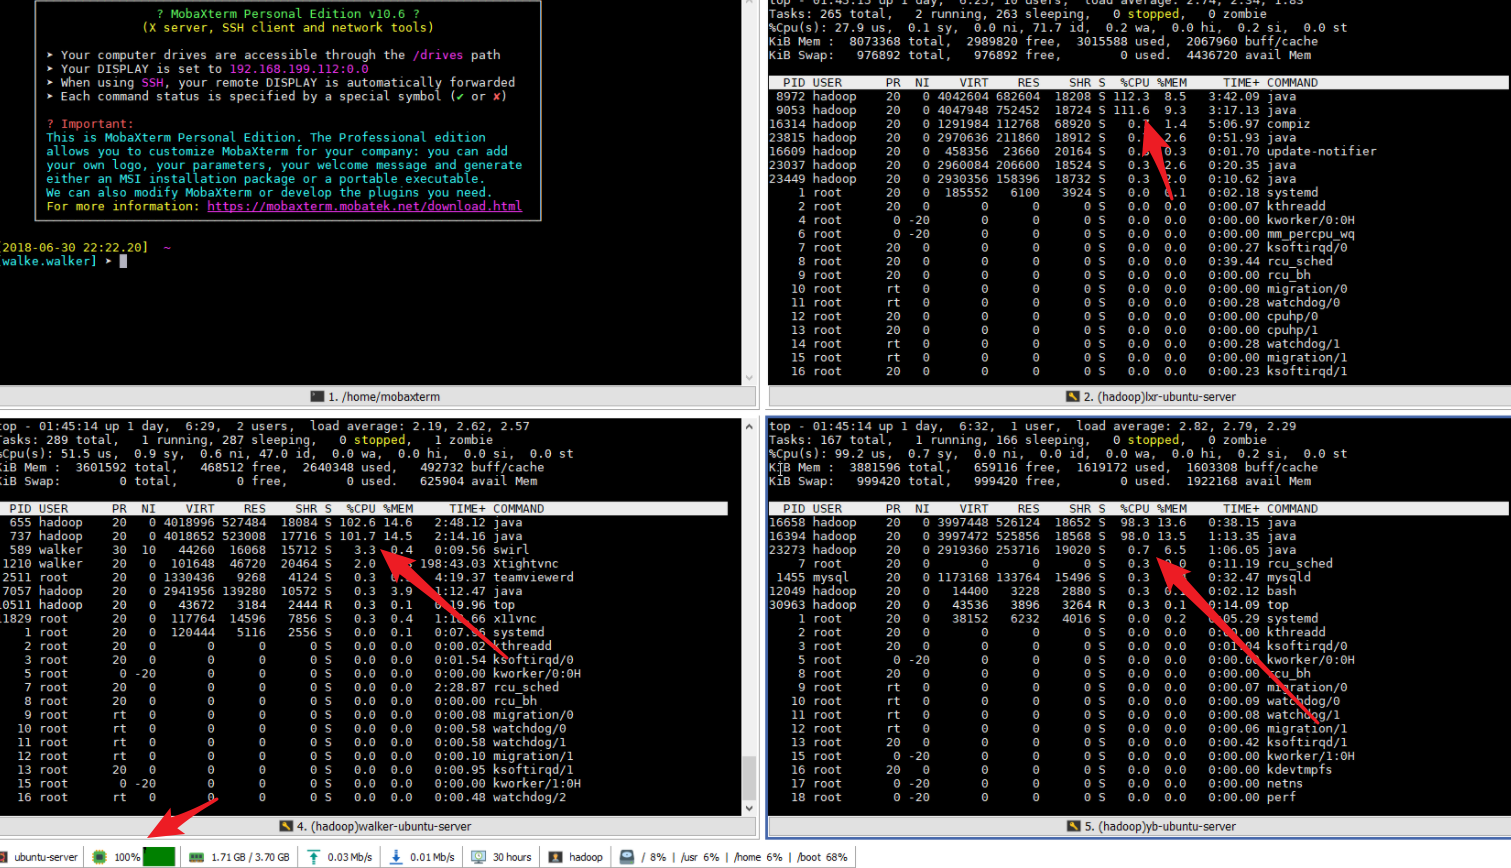
\includegraphics[width=13cm]{"./figure/2018-07-03-14-41-38.png"}
  \caption{在step4计算时三主机的负载情况}
  \label{fig:result-step4-top}
  %\end{adjustwidth}
\end{figure}


%\usepackage{changepage}
%\usepackage{rotating}
%\usepackage{float}
%\usepackage[section]{placeins}
%\begin{sidewaystable}[!Htp]
\begin{figure}[htp]
  %\begin{adjustwidth}{-1.5cm}{-1cm}
  \centering
  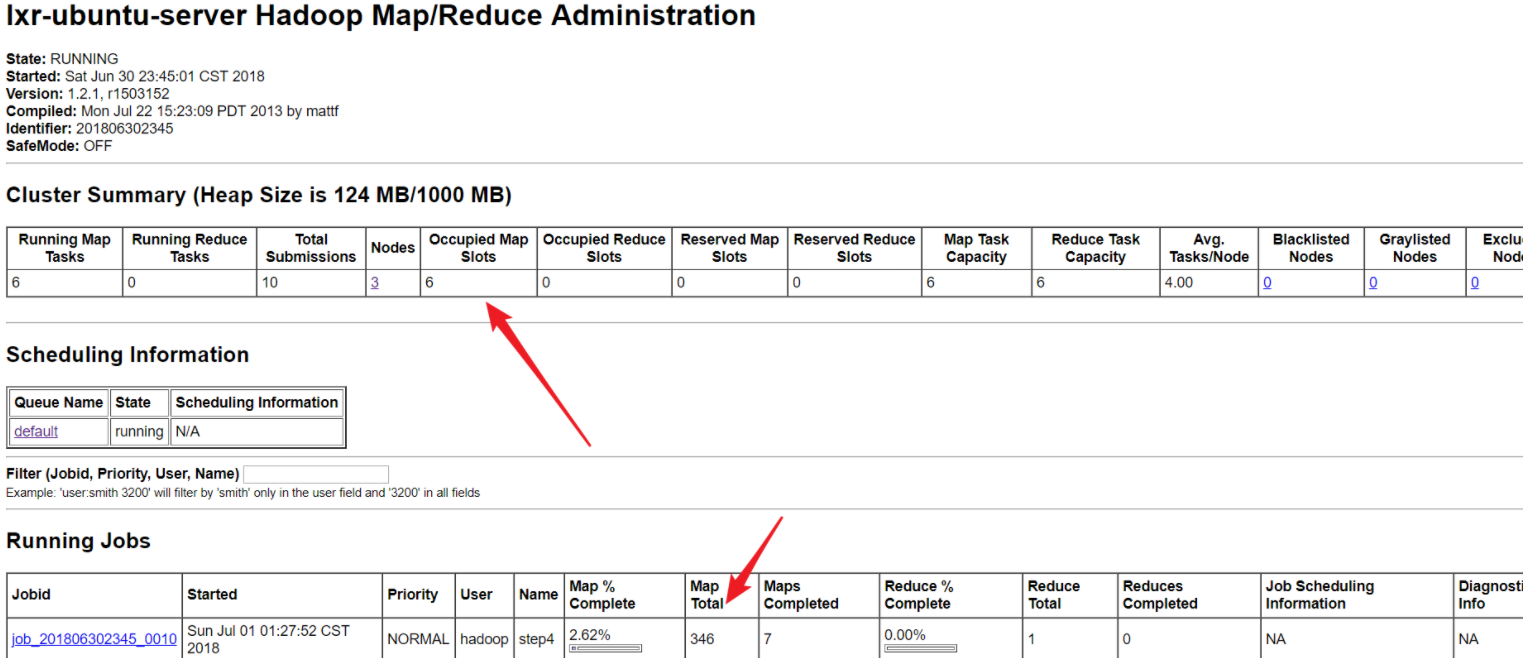
\includegraphics[width=13cm]{"./figure/2018-07-03-14-42-57.png"}
  \caption{在step4计算时jobtracker的情况}
  \label{fig:result-step4-jobtracker}
  %\end{adjustwidth}
\end{figure}

最终花了10个小时完成了这个计算,并且计算的结果可见\autoref{fig:result-all}。其中第一列是用户ID,第二列是“电影ID\_最终得分”。



%\usepackage{changepage}
%\usepackage{rotating}
%\usepackage{float}
%\usepackage[section]{placeins}
%\begin{sidewaystable}[!Htp]
\begin{figure}[htp]
  %\begin{adjustwidth}{-1.5cm}{-1cm}
  \centering
  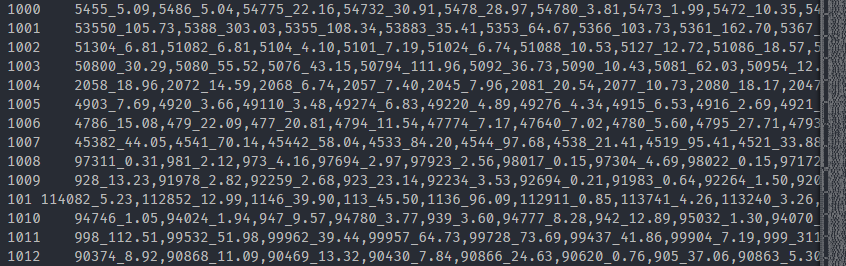
\includegraphics[width=13cm]{"./figure/2018-07-03-14-46-28.png"}
  \caption{运算结果}
  \label{fig:result-all}
  %\end{adjustwidth}
\end{figure}


\chapter{关于性能的思考}

在我们跑数据的时候,我对这个性能有了一些更加深入的思考,以下主要说明两点

\subsection{关于hdfs中block大小的设置}

hadoop底层依附的是hdfs分布式文件系统,这个文件系统能够将文件分布式并且增加冗余备份的存放在不同的节点上,而这一切的细节对用户透明,用户只需要想往常使用linux中的文件系统一样使用hdfs就可以了。

其中,有一个概念与hdfs,及之后hadoop进行计算时的性能息息相关:block 的大小。在hdfs中,默认的block大小为64mb,这意味着小于64mb的文件,仅仅作为一个块,是无法实现分布式计算的。这也是我们一开始测试数据的时候无法实现分布式的并行计算的重要原因。后来,查询相关资料,我知道了如何改变block 的默认大小。这只需要在hadoop的conf中,增加或修改以下属性值就可以了。

%\usepackage{listings}
\begin{lstlisting}[style = c]
<property>
  <name>dfs.block.size</name>
  <value>1048576</value>
</property>
\end{lstlisting}

在将block大小设置为1mb后,我们之后的测试能够看到,即使是只有3mb多一点的测试数据,hadoop也会根据block的大小,将这个任务划分为4个map任务,并将这个任务分发到三台主机上去运行。这样子就真正实现了分布式的计算。关于这个,可见\autoref{fig:result-step4-top}。

当然,这样设置block 的大小并不与hdfs这个文件系统的设计相吻合。hdfs本身是设计为大文件的存储的,因此对于TB级别的数据,PB级别的数据,使用较大的block,能够显著的体验到hdfs对大文件的良好支持。而我们的相对较小的数据,则无法体现出hdfs的优势。


\subsection{关于slot的分配}

hadoop 1.2.1 中有slot的概念。它是这样的,在每一台机子上跑的hadoop,当分发map工作和reduce工作时,是抽象为将工作交给一个slot来做,每个slot有它对应的内存大小,CPU资源等。可以说,slot就是一种计算资源的单位。hadoop将一个工作交给一个单位来完成。

因此,对于性能不同的电脑而言,应该具有不同数量的slot,这样hadoop在进行任务分配,负载均衡的时候,就能够充分利用每一台机的运算力。

之所以研究这个问题,是因为在我们的实验过程中,三台电脑的CPU占用率差别很大。在hadoop默认的每一台机有两个slot中,我们的实验现象也的确是,每一台主机运行只运行两个map任务。但是如果这样的话,我们的集群便会有很多性能被拜拜浪费无法使用了。三台主机的CPU占有率可见\autoref{fig:CPU-diff}。

%\usepackage{changepage}
%\usepackage{rotating}
%\usepackage{float}
%\usepackage[section]{placeins}
%\begin{sidewaystable}[!Htp]
\begin{figure}[htp]
  %\begin{adjustwidth}{-1.5cm}{-1cm}
  \centering
  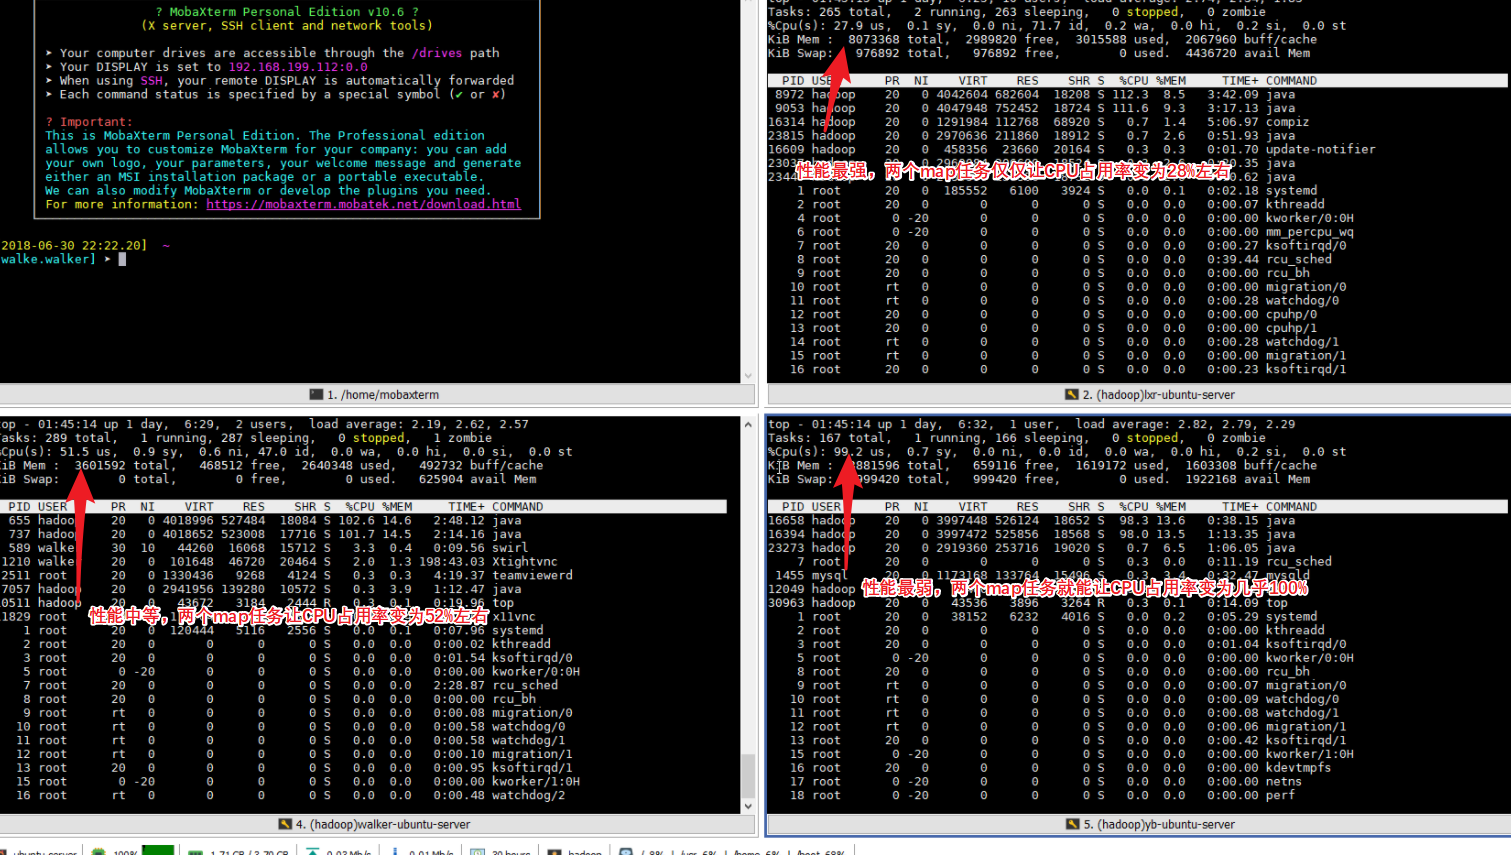
\includegraphics[width=13cm]{"./figure/2018-07-03-15-06-19.png"}
  \caption{三台电脑两个map任务中的CPU占用率对比}
  \label{fig:CPU-diff}
  %\end{adjustwidth}
\end{figure}

关于slot的情况,在hadoop的jobtracker中同样可以看到相关的数据,\autoref{fig:show-jobtracker-slot}可以见到目前系统中总共有6个slot在工作,同时最大的也只能有6个slot工作。这与此前我们每台主机的情况一致。

%\usepackage{changepage}
%\usepackage{rotating}
%\usepackage{float}
%\usepackage[section]{placeins}
%\begin{sidewaystable}[!Htp]
\begin{figure}[htp]
  %\begin{adjustwidth}{-1.5cm}{-1cm}
  \centering
  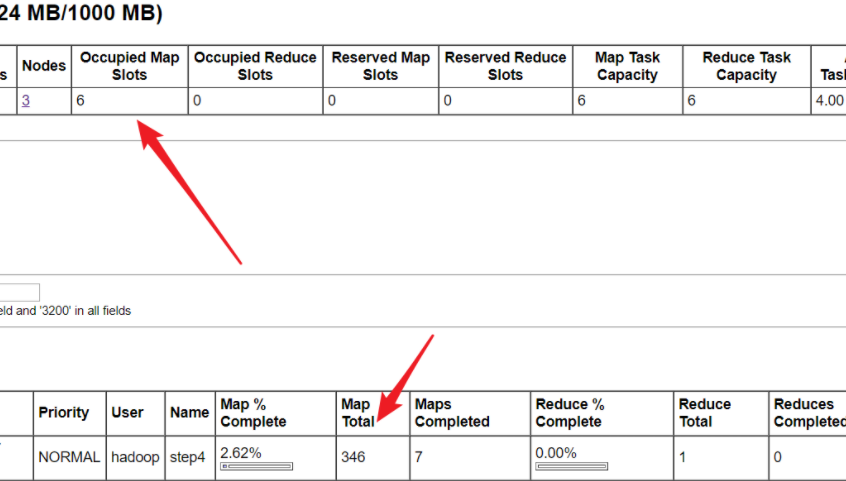
\includegraphics[width=10cm]{"./figure/2018-07-03-15-16-59.png"}
  \caption{在jobtracker中查看slot的情况}
  \label{fig:show-jobtracker-slot}
  %\end{adjustwidth}
\end{figure}





%%%%%%%%%%%%%%%%%%%%%%%%%%%%%%%%%%%%%%%%%%%%%%%%%%%%%%%%%%%%%%%%%%%%%%%%%%%%
% 参考文献
%%%%%%%%%%%%%%%%%%%%%%%%%%%%%%%%%%%%%%%%%%%%%%%%%%%%%%%%%%%%%%%%%%%%%%%%%%%%
\cleardoublepage\phantomsection
\addcontentsline{toc}{chapter}{参考资料}

\bibliography{opsystem}
\bibliographystyle{unsrt}

\begin{thebibliography}{00}
  \bibitem{class1} 慕课网教程:Hadoop大数据平台架构与实践--基础篇,\url{https://www.imooc.com/learn/391}
  \bibitem{class2} 慕课网教程:Hadoop大数据平台架构与实践--进阶篇,\url{https://www.imooc.com/learn/890}
  \bibitem{blog1} Hadoop 1.0与Hadoop 2.0资源管理方案对比,\url{http://dongxicheng.org/mapreduce-nextgen/hadoop-1-and-2-resource-manage/}

\end{thebibliography}
%%%%%%%%%%%%%%%%%%%%%%%%%%%%%%%%%%%%%%%%%%%%%%%%%%%%%%%%%%%%%%%%%%%%%%%%%%%%
% 附录
%%%%%%%%%%%%%%%%%%%%%%%%%%%%%%%%%%%%%%%%%%%%%%%%%%%%%%%%%%%%%%%%%%%%%%%%%%%%
\appendix

\chapter{文件的组织}

\cleardoublepage
\end{document}